\chapter{\textit{Web Services} RESTful e SPAs}\label{cap:webservicesRestful}
\epigraph{``\textit{Não extingua sua inspiração e sua imaginação; não se torne o escravo do seu modelo}''.}{Vincent van Gogh}

\lettrine[lines=4, lhang=0.1, lraise=0, loversize=0.2, findent=0.1em]{\textcolor{corTema}{N}}{ESTE} capítulo vamos revisitar o sistema de vendas de produtos que construímos no capítulo~\ref{cap:sistemaVendaProdutos}, mas sob uma ótica completamente diferente. Desta vez, em vez de um único projeto monolítico em que o servidor gera páginas HTML completas para o navegador, vamos separá-lo em dois projetos independentes: um \textit{back-end} que expõe \textit{Web Services} RESTful, e um \textit{front-end} que é uma \textit{Single Page Application} (SPA) construída com JavaScript puro, sem nenhum \textit{framework}.

\vfill

\section{Introdução}

Até aqui, toda vez que o usuário realizava uma ação no sistema --- clicar em ``Salvar'', ``Excluir'', navegar entre páginas --- o navegador disparava uma requisição HTTP, o servidor processava essa requisição, montava uma página HTML completa com todos os seus dados e a devolvia para o navegador recarregar. Esse modelo, chamado de \destaque{renderização no servidor} (\textit{server-side rendering}), é extremamente simples e funciona muito bem para muitos casos. Foi exatamente o que aprendemos nos capítulos anteriores.

Mas imagine agora que nosso sistema de vendas precisasse ser consumido também por um aplicativo mobile, ou por um sistema de terceiros que queira integrar nossos dados. Nesse cenário, o servidor gerar HTML não faz sentido algum --- um aplicativo mobile não renderiza HTML como um navegador. O que todos esses clientes diferentes têm em comum é a capacidade de entender dados estruturados. E o formato que se tornou o padrão universal para essa troca de dados é o JSON.

É aí que entram os \textit{Web Services} RESTful. Em vez de o servidor gerar HTML, ele passa a expor \textbf{recursos} (estados, cidades, produtos, vendas\ldots) através de uma interface bem definida usando os verbos do próprio protocolo HTTP, devolvendo e recebendo dados em JSON. Qualquer cliente que saiba fazer requisições HTTP e interpretar JSON pode consumi-lo --- seja um navegador, um app mobile, ou outro sistema.

Neste capítulo construiremos um projeto separado em duas partes: o \texttt{backend}, implantado no Apache Tomcat, que expõe os serviços RESTful, e o \texttt{frontend}, servido pelo Vite durante o desenvolvimento, que é uma SPA capaz de realizar todas as operações do sistema consumindo esses serviços.

\begin{saibaMais}
    O Vite é uma ferramenta de \textit{build} e servidor de desenvolvimento para aplicações Web modernas. Em modo de desenvolvimento ele serve os arquivos estáticos com atualizações instantâneas. Para este capítulo usamos o Vite apenas para servir o \textit{front-end} em \texttt{http://localhost:5173} durante o desenvolvimento, sem nenhum \textit{framework} JavaScript adicional.
\end{saibaMais}


\section{O que é REST?}

REST (\textit{Representational State Transfer}) é um estilo arquitetural proposto por Roy Fielding em sua tese de doutorado em 2000. Não é um protocolo, não é um padrão formal --- é um conjunto de restrições arquiteturais que, quando seguidas, resultam em serviços escaláveis, simples e interoperáveis.

Os princípios centrais que nos interessam são:

\begin{itemize}
    \item \textbf{Recursos identificados por URIs}: cada entidade do sistema tem um endereço único. \texttt{/api/estados} representa a coleção de estados, \texttt{/api/estados/7} representa o estado de id 7.
    \item \textbf{Manipulação através de verbos HTTP}: usamos GET para listar/buscar, POST para criar, PUT para atualizar e DELETE para remover. O protocolo HTTP já tem esses verbos; REST apenas os usa com semântica precisa.
    \item \textbf{\textit{Stateless}}: cada requisição é autocontida. O servidor não guarda estado de sessão entre requisições. Toda informação necessária para processar a requisição deve estar nela mesma.
    \item \textbf{Representação negociada}: o mesmo recurso pode ser representado de formas diferentes. Usaremos JSON, mas o protocolo prevê outros formatos.
\end{itemize}

A Tabela~\ref{tab:cap10VerbosHTTP} mostra o mapeamento que adotamos no nosso sistema entre verbos HTTP, URIs e operações CRUD.

\begin{table}[!htbp]
\centering
\caption{Mapeamento de verbos HTTP para operações CRUD}
\label{tab:cap10VerbosHTTP}
\begin{tabular}{llll}
\hline
\textbf{Verbo} & \textbf{URI} & \textbf{Operação} & \textbf{Status de sucesso} \\
\hline
GET    & \texttt{/api/estados}    & Listar todos      & 200 OK         \\
GET    & \texttt{/api/estados/7} & Buscar por id     & 200 OK         \\
POST   & \texttt{/api/estados}    & Inserir           & 201 Created    \\
PUT    & \texttt{/api/estados/7} & Atualizar         & 200 OK         \\
DELETE & \texttt{/api/estados/7} & Excluir           & 200 OK         \\
\hline
\end{tabular}
\\\textbf{Fonte:} Elaborada pelo autor
\end{table}

\begin{saibaMais}
    Os códigos de status HTTP são divididos em classes: \textbf{2xx} indicam sucesso (200 OK, 201 Created, 204 No Content); \textbf{3xx} indicam redirecionamento; \textbf{4xx} indicam erros do cliente (400 Bad Request para dados inválidos, 404 Not Found para recurso inexistente, 405 Method Not Allowed para verbo não suportado); \textbf{5xx} indicam erros do servidor (500 Internal Server Error para erros inesperados). Em serviços RESTful é fundamental retornar o status correto, pois os clientes tomam decisões com base nele --- um status 400 significa ``corrija seus dados e tente novamente'', enquanto um 500 significa ``problema no servidor, tente mais tarde''.
\end{saibaMais}


\section{O Projeto}

O projeto deste capítulo mantém exatamente as mesmas entidades, DAOs e base de dados do capítulo~\ref{cap:sistemaVendaProdutos}. O que muda profundamente é a camada de controle: em vez de Servlets que geram HTML via \texttt{RequestDispatcher}, temos Servlets que recebem e devolvem JSON. O \textit{front-end} HTML/CSS/JS foi completamente reescrito como uma SPA.

Você pode pegar os dois projetos prontos nos arquivos deste capítulo. A estrutura de pacotes do \textit{back-end} pode ser vista na Figura~\ref{fig:cap10EstruturaPacotes}.

\FloatBarrier
\begin{figure}[!htbp]
    \centering
    \caption{Estrutura de pacotes do \textit{back-end}}
    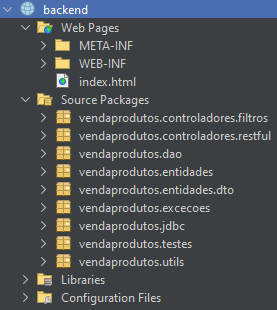
\includegraphics[scale=0.6]{imagens/cap10EstruturaPacotes}
    \\\textbf{Fonte:} Elaborada pelo autor
    \label{fig:cap10EstruturaPacotes}
\end{figure}
\FloatBarrier

Note que o pacote \texttt{controladores} agora contém apenas dois subpacotes: \texttt{filtros} (onde ficam os filtros de servlet) e \texttt{restful} (onde ficam nossos Servlets RESTful). Não há mais JSPs, não há mais páginas HTML no lado do servidor --- tudo o que o \textit{back-end} devolve é JSON.

\subsection{Dois Projetos, Duas Ferramentas}

Uma das diferenças práticas desse modelo de separação é que \textit{back-end} e \textit{front-end} são projetos completamente independentes, podendo ser desenvolvidos com ferramentas diferentes. Neste livro, o projeto \texttt{backend} é um projeto NetBeans convencional, implantado no Apache Tomcat exatamente como nos capítulos anteriores. O projeto \texttt{frontend}, por outro lado, não tem nenhuma dependência de IDE específica: é uma pasta com arquivos JavaScript, HTML e CSS que pode ser aberta em qualquer editor.

Para executar o sistema você precisa ter os dois em funcionamento ao mesmo tempo. O \textit{back-end} é iniciado pelo NetBeans como sempre (botão ``\textit{Run Project}'', que implanta o projeto no Tomcat e o inicia). O \textit{front-end} precisa apenas de um servidor HTTP local para servir os arquivos estáticos --- nada de compilação ou ferramentas de \textit{build}. A forma mais simples de fazer isso no Visual Studio Code (\url{https://code.visualstudio.com}) é instalar a extensão \textit{Live Server} e clicar em ``Go Live'' na barra de status. O \textit{front-end} ficará disponível em \texttt{http://localhost:5500} (ou porta similar) e fará requisições ao \textit{back-end} em \texttt{http://localhost:8080}.


\subsection{CORS --- \textit{Cross-Origin Resource Sharing}}

Antes de ver qualquer Servlet RESTful, precisamos entender um problema que inevitavelmente enfrentamos quando separamos o \textit{front-end} do \textit{back-end} em origens diferentes.

A política de mesma origem (\textit{Same-Origin Policy}) é uma medida de segurança dos navegadores que impede que JavaScript em execução em uma página de uma origem (combinação de esquema, domínio e porta) faça requisições para outra origem sem permissão explícita. No nosso caso, o \textit{front-end} está em \texttt{http://localhost:5173} e o \textit{back-end} está em \texttt{http://localhost:8080}. Portas diferentes --- origens diferentes. Sem nenhuma configuração adicional, o navegador bloqueará todas as requisições do \textit{front-end} para o \textit{back-end}.

CORS é o mecanismo que permite que o servidor diga ao navegador quem tem permissão para acessá-lo. Isso é feito através de cabeçalhos HTTP especiais. Além das requisições normais, o navegador às vezes envia antes uma requisição de \destaque{\textit{preflight}} (método \texttt{OPTIONS}) para perguntar ao servidor o que é permitido. O servidor deve responder a essa requisição com os cabeçalhos corretos ou o navegador bloqueará a requisição real.

No nosso projeto implementamos o filtro \texttt{CORSFilter}, mostrado na Listagem~\thechapter.\ref{listagem:projetos/capitulo10/VendaProdutosSPA/backend/src/java/vendaprodutos/controladores/filtros/CORSFilter.java}, que cuida de tudo isso.

\javaCode{Filtro CORS\newline%
Arquivo: \texttt{vendaprodutos/controladores/filtros/CORSFilter.java}}{projetos/capitulo10/VendaProdutosSPA/backend/src/java/vendaprodutos/controladores/filtros/CORSFilter.java}

Veja que na linha 18 o filtro é configurado para interceptar qualquer requisição cujo caminho comece com \texttt{/api/*}, que é exatamente o prefixo de todos os nossos Servlets RESTful. Independentemente do que for requisitado, esse filtro sempre rodará primeiro.

A constante \inlineJavaCode{BLOQUEAR_POR_DOMINIO} na linha 21 controla o comportamento do cabeçalho \texttt{Access-Control-Allow-Origin}. Quando \inlineJavaCode{false}, o cabeçalho é configurado com \texttt{*} (linha 35), o que significa que qualquer origem pode fazer requisições ao servidor. Isso é adequado para desenvolvimento e para APIs públicas. Quando \inlineJavaCode{true} (linhas 37 a 41), o servidor verifica se a origem da requisição está em uma lista de permitidas e, somente nesse caso, devolve a origem no cabeçalho --- o que é o comportamento correto para sistemas em produção.

Os outros cabeçalhos (linhas 42 a 44) definem quais métodos HTTP são permitidos, quais cabeçalhos podem ser enviados nas requisições e por quanto tempo o resultado do \textit{preflight} pode ser cacheado pelo navegador (3600 segundos = 1 hora).

Por fim, entre as linhas 47 e 50, o filtro verifica se a requisição é um \textit{preflight} (método \texttt{OPTIONS}). Se for, responde imediatamente com status 200 e encerra sem passar para a cadeia de filtros --- o que é o comportamento correto, pois o Servlet não deveria nem ver uma requisição de \textit{preflight}.

\begin{atencao}
    Com \inlineJavaCode{BLOQUEAR_POR_DOMINIO = false} e \texttt{Access-Control-Allow-Origin: *}, qualquer site na internet pode fazer requisições ao seu servidor. Em desenvolvimento isso é conveniente, mas em produção você deve sempre restringir às origens conhecidas e confiáveis.
\end{atencao}


\subsection{A Resposta Padronizada}

Para que todos os Servlets RESTful devolvam respostas em um formato consistente, criamos o \textit{record} \texttt{Resposta}, apresentado na Listagem~\thechapter.\ref{listagem:projetos/capitulo10/VendaProdutosSPA/backend/src/java/vendaprodutos/controladores/restful/Resposta.java}.

\javaCode{\textit{Record} \texttt{Resposta}\newline%
Arquivo: \texttt{vendaprodutos/controladores/restful/Resposta.java}}{projetos/capitulo10/VendaProdutosSPA/backend/src/java/vendaprodutos/controladores/restful/Resposta.java}

Simples assim. Todo JSON que o servidor devolve terá dois campos: \texttt{mensagem} (uma \texttt{String} descrevendo o resultado da operação) e \texttt{dados} (o objeto que foi criado, atualizado ou consultado --- ou uma \textit{string} vazia em caso de erro). No \textit{front-end} sempre saberemos como interpretar a resposta, pois o formato é sempre o mesmo.

\begin{saibaMais}
    \textit{Records} são uma funcionalidade do Java 16+ que permitem criar classes imutáveis de transporte de dados de forma extremamente concisa. Um \textit{record} automaticamente gera o construtor, os acessores (com o mesmo nome dos campos), \texttt{equals}, \texttt{hashCode} e \texttt{toString}. São ideais para objetos que apenas carregam dados, como os nossos DTOs e a classe \texttt{Resposta}.
\end{saibaMais}


\subsection{Utilitários do \textit{Back-End}}

Antes de vermos os Servlets, há dois métodos da classe \texttt{Utils} que são novos neste projeto e fundamentais para o funcionamento dos serviços RESTful.

\javaCode{Classe \texttt{Utils} com os novos métodos\newline%
Arquivo: \texttt{vendaprodutos/utils/Utils.java}}{projetos/capitulo10/VendaProdutosSPA/backend/src/java/vendaprodutos/utils/Utils.java}

O método \inlineJavaCode{obterDados} (linha 236) lê o corpo completo da requisição HTTP como uma \texttt{String}. Em vez de parâmetros de formulário (como nos capítulos anteriores, onde usávamos \inlineJavaCode{request.getParameter(...)}), os Servlets RESTful recebem os dados como JSON no corpo da requisição. Esse método encapsula a leitura desse corpo linha a linha usando um \texttt{BufferedReader}.

O método \inlineJavaCode{validar} (linha 190) é praticamente o mesmo do capítulo~\ref{cap:sistemaVendaProdutos}, mas com uma diferença crucial: em vez de lançar \texttt{SQLException}, agora lança \inlineJavaCode{ValidacaoException}, que é uma exceção não verificada (\textit{unchecked}) de nossa autoria. Isso permite que a exceção de validação se propague naturalmente pelos métodos dos DAOs (que lançam \texttt{SQLException}) sem precisar ser declarada em suas assinaturas. As classes de exceção são apresentadas nas Listagens~\thechapter.\ref{listagem:projetos/capitulo10/VendaProdutosSPA/backend/src/java/vendaprodutos/excecoes/ValidacaoException.java} e~\thechapter.\ref{listagem:projetos/capitulo10/VendaProdutosSPA/backend/src/java/vendaprodutos/excecoes/NaoEncontradoException.java}.

\javaCode{\texttt{ValidacaoException}\newline%
Arquivo: \texttt{vendaprodutos/excecoes/ValidacaoException.java}}{projetos/capitulo10/VendaProdutosSPA/backend/src/java/vendaprodutos/excecoes/ValidacaoException.java}

\javaCode{\texttt{NaoEncontradoException}\newline%
Arquivo: \texttt{vendaprodutos/excecoes/NaoEncontradoException.java}}{projetos/capitulo10/VendaProdutosSPA/backend/src/java/vendaprodutos/excecoes/NaoEncontradoException.java}

Ambas estendem \inlineJavaCode{RuntimeException}, que é a superclasse de todas as exceções não verificadas do Java. Ao usar exceções não verificadas nos nossos Servlets podemos adicionar blocos \inlineJavaCode{catch} específicos para cada tipo de problema (validação $\rightarrow$ 400, não encontrado $\rightarrow$ 404, SQL $\rightarrow$ 500) sem que os métodos dos DAOs precisem conhecer ou declarar essas exceções.


\section{Os Servlets RESTful}

Todos os nossos Servlets RESTful seguem a mesma estrutura básica: sobreescrevem os métodos \inlineJavaCode{doGet}, \inlineJavaCode{doPost}, \inlineJavaCode{doPut} e \inlineJavaCode{doDelete} do \texttt{HttpServlet}. Em cada método, a estrutura interna é:

\begin{enumerate}
    \item Configurar o tipo de conteúdo da resposta como \texttt{application/json}.
    \item Dentro de um bloco \textit{try-with-resources} com o(s) DAO(s) necessário(s), executar a operação.
    \item Em caso de sucesso, construir um \texttt{Resposta} com mensagem e dados, serializá-lo com o JSON-B e configurar o status HTTP apropriado.
    \item Em blocos \inlineJavaCode{catch} específicos, capturar \inlineJavaCode{ValidacaoException} ($\rightarrow$ 400), \inlineJavaCode{NaoEncontradoException} ($\rightarrow$ 404), \texttt{SQLException} ($\rightarrow$ 500) e \texttt{NumberFormatException} ($\rightarrow$ 400 quando o ID da URL não é numérico).
    \item Escrever o JSON na resposta.
\end{enumerate}

O campo \inlineJavaCode{jsonb} declarado em cada Servlet (linha 27 do \texttt{EstadoRestfulServlet}) é uma instância de \inlineJavaCode{Jsonb}, a interface principal da API Jakarta JSON-B. Com ela, \inlineJavaCode{jsonb.toJson(objeto)} serializa qualquer objeto Java para JSON e \inlineJavaCode{jsonb.fromJson(string, Classe.class)} faz o caminho inverso.

\begin{saibaMais}
    A Jakarta JSON-B (\textit{JSON Binding}) é a especificação padrão do Jakarta EE para mapeamento entre objetos Java e JSON. Ela funciona de forma similar ao JAXB para XML: usa reflexão para inspecionar os campos e acessores do objeto e gera o JSON correspondente. A implementação de referência é o Yasson. Por padrão, ela usa os nomes dos campos Java como nomes das propriedades JSON, o que em nosso caso é exatamente o comportamento desejado.
\end{saibaMais}


\subsection{O Servlet de Estados --- Um CRUD Completo}

Começaremos com o Servlet mais simples, o \texttt{EstadoRestfulServlet}, pois estados não têm dependências com outras entidades. Sua implementação completa é apresentada na Listagem~\thechapter.\ref{listagem:projetos/capitulo10/VendaProdutosSPA/backend/src/java/vendaprodutos/controladores/restful/EstadoRestfulServlet.java}.

\javaCode{Servlet RESTful para Estados\newline%
Arquivo: \texttt{vendaprodutos/controladores/restful/EstadoRestfulServlet.java}}{projetos/capitulo10/VendaProdutosSPA/backend/src/java/vendaprodutos/controladores/restful/EstadoRestfulServlet.java}

Vamos percorrer cada método.

\subsubsection{doGet --- Listagem e Busca por ID}

A anotação \inlineJavaCode{@WebServlet} na linha 24 mapeia este Servlet para \texttt{/api/estados/*}. O asterisco significa que qualquer caminho que comece com \texttt{/api/estados/} também será tratado por ele. Isso nos permite usar um único Servlet para tanto a listagem (\texttt{GET /api/estados/}) quanto a busca por id (\texttt{GET /api/estados/7}).

Dentro do \inlineJavaCode{doGet} (linha 30), a distinção entre os dois casos é feita pelo \inlineJavaCode{pathInfo} (linha 40). Quando a URL é apenas \texttt{/api/estados/}, o \inlineJavaCode{pathInfo} é \inlineJavaCode{null} ou \texttt{"/"}. Quando há um id, como em \texttt{/api/estados/7}, o \inlineJavaCode{pathInfo} é \texttt{"/7"}. Neste último caso (linha 45), extraímos o id removendo a barra inicial com \inlineJavaCode{substring(1)} e convertemos para \texttt{Long}. Se o estado existir, devolvemos ele serializado diretamente (linha 50) --- sem o envelope \texttt{Resposta}, pois neste caso o JSON do estado já é a resposta completa. Se não existir (linha 52), devolvemos um \texttt{Resposta} com status 404.

Para a listagem (linha 59), simplesmente devolvemos a lista inteira serializada como um array JSON.

\subsubsection{doPost --- Inserção}

No \inlineJavaCode{doPost} (linha 78), o JSON com os dados do novo estado vem no corpo da requisição. Usamos \inlineJavaCode{Utils.obterDados(request)} para ler esse corpo como \texttt{String} e então o \inlineJavaCode{jsonb.fromJson(...)} para desserializá-lo para um objeto \texttt{Estado} (linhas 88 a 91).

Em seguida, validamos o objeto com \inlineJavaCode{Utils.validar(estado, "id")} (linha 93) ignorando o campo \texttt{id}, pois um estado novo ainda não tem identificador. Se a validação falhar, \inlineJavaCode{ValidacaoException} será lançada e capturada pelo \inlineJavaCode{catch} da linha 100, resultando em uma resposta 400 com a descrição dos erros. Se tudo estiver correto, o estado é salvo (linha 94) e respondemos com status 201 (Created), adicionando o cabeçalho \texttt{Location} com o endereço do novo recurso.

\subsubsection{doPut --- Atualização}

No \inlineJavaCode{doPut} (linha 116), a URL inclui o id do estado a ser atualizado (ex.: \texttt{PUT /api/estados/7}) e o corpo da requisição contém os novos dados.

O ponto mais importante aqui é que não atualizamos cegamente o objeto recebido --- primeiro buscamos o estado existente no banco de dados pelo id (linha 134). Se ele não existir, lançamos \inlineJavaCode{NaoEncontradoException} (linha 137), que resulta em uma resposta 404. Isso é fundamental: precisamos do objeto existente para garantir que não estamos sobrescrevendo campos que o cliente não enviou. Só então transferimos os novos valores (linhas 140 e 141) e validamos/atualizamos.

\subsubsection{doDelete --- Exclusão}

O \inlineJavaCode{doDelete} (linha 171) é o mais simples. Extraímos o id da URL, buscamos o estado e chamamos \inlineJavaCode{dao.excluir(estado)}. Aqui não adicionamos verificação de nulo antes da exclusão porque, se o estado não existir, o DAO tentará excluir um objeto nulo e lançará \texttt{SQLException}, que cai no \inlineJavaCode{catch} de erros do servidor. Isso poderia ser melhorado com um \inlineJavaCode{NaoEncontradoException}, mas optamos por manter o exemplo simples.


\subsection{O Servlet de Produtos --- Múltiplos DAOs no PUT}

O Servlet de produtos segue a mesma estrutura do de estados, mas com uma peculiaridade interessante no \inlineJavaCode{doPut}: um produto tem dependências com fornecedor e unidade de medida, e precisamos verificar se houve mudanças nesses relacionamentos para buscar os objetos completos no banco.

\javaCode{Servlet RESTful para Produtos\newline%
Arquivo: \texttt{vendaprodutos/controladores/restful/ProdutoRestfulServlet.java}}{projetos/capitulo10/VendaProdutosSPA/backend/src/java/vendaprodutos/controladores/restful/ProdutoRestfulServlet.java}

Veja o \inlineJavaCode{doPut} (linha 118). Três DAOs são abertos no \textit{try-with-resources} (linhas 126 a 128): um para produtos, um para fornecedores e um para unidades de medida. Após buscar o produto existente (linha 138) e verificar que ele existe (linha 140), atualizamos os campos simples (linhas 144 a 148). Mas para os relacionamentos (linhas 149 a 155), verificamos se o fornecedor ou a unidade de medida enviados pelo cliente são diferentes dos que o produto já tem, usando o método \inlineJavaCode{equals}. Só se houver mudança fazemos a consulta ao banco para obter o objeto completo. Essa verificação evita buscas desnecessárias ao banco de dados.


\subsection{O Servlet de Vendas --- DTOs e Sub-recursos}

O Servlet de vendas é o mais complexo do projeto. Vamos examiná-lo na Listagem~\thechapter.\ref{listagem:projetos/capitulo10/VendaProdutosSPA/backend/src/java/vendaprodutos/controladores/restful/VendaRestfulServlet.java}.

\javaCode{Servlet RESTful para Vendas\newline%
Arquivo: \texttt{vendaprodutos/controladores/restful/VendaRestfulServlet.java}}{projetos/capitulo10/VendaProdutosSPA/backend/src/java/vendaprodutos/controladores/restful/VendaRestfulServlet.java}

\subsubsection{O Problema da Inserção de Vendas}

No \inlineJavaCode{doPost} (linha 87), criar uma venda envolve mais do que os dados de uma única entidade. O cliente precisa enviar o id do cliente e uma lista de itens, cada um com o id do produto e a quantidade. Não podemos usar a classe \texttt{Venda} diretamente para desserialização porque ela contém um objeto \texttt{Cliente} completo e uma lista de \texttt{ItemVenda} que só faz sentido após a venda ser criada.

A solução é usar um \textbf{DTO} (\textit{Data Transfer Object}). Criamos dois \textit{records} específicos para receber os dados do cliente:

\javaCode{DTO para recebimento de vendas\newline%
Arquivo: \texttt{vendaprodutos/entidades/dto/VendaDTO.java}}{projetos/capitulo10/VendaProdutosSPA/backend/src/java/vendaprodutos/entidades/dto/VendaDTO.java}

\javaCode{DTO para recebimento de itens de venda\newline%
Arquivo: \texttt{vendaprodutos/entidades/dto/ItemVendaDTO.java}}{projetos/capitulo10/VendaProdutosSPA/backend/src/java/vendaprodutos/entidades/dto/ItemVendaDTO.java}

O JSON enviado pelo \textit{front-end} para criar uma venda tem a seguinte forma:

\begin{lstlisting}[language=java, caption={Exemplo de JSON para criação de venda}]
{
    "idCliente": 3,
    "itens": [
        { "idProduto": 12, "quantidade": 2 },
        { "idProduto": 5,  "quantidade": 1.5 }
    ]
}
\end{lstlisting}

O JSON-B desserializa esse JSON diretamente em um objeto \texttt{VendaDTO} (linhas 100 a 102 do Servlet). A partir desse DTO, o Servlet constrói os objetos do domínio: busca o cliente pelo id (linha 104), cria a venda com a data atual (linhas 106 a 110), salva a venda (linha 112) e então itera sobre os itens para criar cada \texttt{ItemVenda}, atualizando o estoque do produto no processo (linhas 114 a 128).

\subsubsection{O Cancelamento --- Sub-recurso via PUT}

Cancelar uma venda não é exatamente uma atualização de recurso --- é uma ação. Uma abordagem RESTful comum para isso é criar um sub-recurso que representa essa ação: \texttt{PUT /api/vendas/cancelar/7} cancela a venda de id 7.

No \inlineJavaCode{doPut} (linha 152), o \inlineJavaCode{pathInfo} pode ser \texttt{/cancelar/7}, que é o único caso que suportamos. Se o caminho começar com \texttt{"/cancelar/"} (linha 166), extraímos o id, buscamos a venda, marcamos como cancelada e devolvemos os itens ao estoque (linhas 170 a 178). Se o caminho for qualquer outra coisa, respondemos com 400 (linha 184).

\begin{saibaMais}
    Em APIs REST mais formais, ações como ``cancelar'' costumam ser modeladas de formas diferentes por diferentes equipes. Algumas usam \texttt{PATCH} (atualização parcial do recurso), outras criam sub-recursos (\texttt{/vendas/7/cancelamento}), outras preferem um \textit{endpoint} de ação explícito. Nenhuma dessas abordagens é errada --- o importante é ser consistente em toda a API.
\end{saibaMais}


\section{A \textit{Single Page Application}}

Agora que o \textit{back-end} está explicado, vamos para o \textit{front-end}. Antes, porém, precisamos entender o que é uma SPA e por que decidimos construir o \textit{front-end} dessa forma.

\subsection{Renderização no Servidor vs. Renderização no Cliente}

No modelo clássico que usamos nos capítulos anteriores, o servidor é responsável por gerar o HTML completo de cada página. Quando o usuário clica em um link ou envia um formulário, o navegador faz uma nova requisição, o servidor processa tudo, gera a página HTML e a envia de volta. O navegador joga fora a página atual e exibe a nova. Esse modelo é chamado de \destaque{renderização no servidor} (\textit{server-side rendering}).

Em uma SPA, o servidor entrega ao navegador uma única página HTML (daí o nome \textit{Single Page Application}) com referências aos arquivos JavaScript. A partir daí, toda a navegação, toda a exibição e atualização de conteúdo acontecem no próprio navegador, sem recarregar a página. Quando o usuário clica em um item de menu, JavaScript intercede, carrega o conteúdo necessário via requisições assíncronas ao servidor, e atualiza apenas a parte da página que precisa mudar. Isso é chamado de \destaque{renderização no cliente} (\textit{client-side rendering}).

Cada abordagem tem seus prós e contras. Renderização no servidor é mais simples de implementar, funciona mesmo sem JavaScript e é favorável para SEO (\textit{Search Engine Optimization}), pois os motores de busca recebem HTML completo. A renderização no cliente resulta em interfaces mais fluídas e responsivas (sem o \textit{flash} branco de recarregamento de página), reduz a carga no servidor (que apenas fornece dados, não HTML) e é o modelo natural quando o \textit{back-end} precisa ser consumido por múltiplos tipos de clientes.

\subsection{Carregamento de Fragmentos HTML}

Nossa SPA não carrega o HTML de cada cadastro de uma vez só. Em vez disso, cada CRUD tem seu HTML armazenado em um arquivo \destaque{fragmento}, e esses fragmentos são carregados sob demanda quando o usuário navega até aquela seção. Esse padrão reduz o tempo de carregamento inicial da aplicação e é a versão manual do que \textit{frameworks} como React, Vue e Angular fazem automaticamente com seus roteadores e sistemas de componentes.

\subsection{JavaScript Puro vs. \textit{Frameworks}}

Toda a implementação do \textit{front-end} deste projeto usa JavaScript puro, sem nenhuma biblioteca ou \textit{framework} adicional. \textit{Frameworks} como React, Vue e Angular existem precisamente para facilitar o desenvolvimento de SPAs: eles gerenciam automaticamente o estado da aplicação, cuidam da atualização eficiente do DOM, fornecem sistemas de roteamento, componentização e muito mais.

Mas essa facilidade tem um custo. \textit{Frameworks} introduzem camadas de abstração que escondem o que acontece por baixo, podem ter curvas de aprendizado consideráveis e, dependendo do tamanho do projeto, podem impactar o desempenho e o tamanho do \textit{bundle} final. Para entender o que um \textit{framework} faz por você, é fundamental ter vivenciado os problemas que ele resolve. É exatamente isso que este capítulo propõe: construir a SPA ``na raça'', gerenciando manualmente o estado dos módulos, o carregamento de fragmentos e o roteamento via menu.

\begin{saibaMais}
    Entre os \textit{frameworks} JavaScript mais populares estão React (mantido pelo Meta), Vue.js (independente) e Angular (mantido pelo Google). Cada um tem sua filosofia e casos de uso ideais. React é uma biblioteca de componentes de UI; Vue é mais opinativo e progressivo; Angular é um \textit{framework} completo com opinião sobre tudo, de roteamento a formulários. Todos resolvem os mesmos problemas fundamentais que enfrentamos neste capítulo, mas de formas diferentes e com diferentes compromissos.
\end{saibaMais}


\section{A Arquitetura do \textit{Front-End}}

O \textit{front-end} é organizado em módulos ES (\textit{ECMAScript Modules}), o sistema oficial de módulos do JavaScript moderno. Cada arquivo \texttt{.js} é um módulo que pode exportar funções, classes ou valores e importar os de outros módulos. As importações do \textit{front-end} seguem o padrão de importar o namespace inteiro: \inlineJavaScriptCode{import * as Utils from "./utils.js"} importa tudo que \texttt{utils.js} exporta e disponibiliza sob o objeto \texttt{Utils}, o que torna o código mais legível ao deixar claro de onde cada função vem.

\begin{saibaMais}
    Antes dos módulos ES se tornarem padrão, o JavaScript não tinha um sistema de módulos nativo. Os desenvolvedores usavam \textit{workarounds} como o padrão IIFE (\textit{Immediately Invoked Function Expression}) ou sistemas como CommonJS (usado no Node.js) e AMD. Hoje, módulos ES são suportados nativamente por todos os navegadores modernos. A sintaxe é simples: \inlineJavaScriptCode{export function minhaFuncao() \{ ... \}} exporta uma função, e \inlineJavaScriptCode{import \{ minhaFuncao \} from "./meuModulo.js"} a importa. Também podemos usar \inlineJavaScriptCode{import * as Nome from "./modulo.js"} para importar tudo de um módulo como um objeto.
\end{saibaMais}


\subsection{O Módulo de Utilitários --- \texttt{utils.js}}

O módulo \texttt{utils.js} é o coração do \textit{front-end}. Ele contém funções utilitárias usadas por todos os outros módulos. Vamos ver as mais importantes na Listagem~\thechapter.\ref{listagem:projetos/capitulo10/VendaProdutosSPA/frontend/src/js/modulos/utils.js}.

\javaScriptCode{Módulo de utilitários\newline%
Arquivo: \texttt{src/js/modulos/utils.js}}{projetos/capitulo10/VendaProdutosSPA/frontend/src/js/modulos/utils.js}

\subsubsection{customFetch --- Requisições com Timeout}

A função \inlineJavaScriptCode{customFetch} (linha 41) é um invólucro ao redor da \textit{Fetch API} nativa do navegador. A \textit{Fetch API} é a forma moderna de fazer requisições HTTP em JavaScript, substituindo o antigo \texttt{XMLHttpRequest}.

O primeiro problema que \inlineJavaScriptCode{customFetch} resolve é o \textit{timeout}. A \textit{Fetch API} nativa não tem suporte a \textit{timeout} --- uma requisição pode ficar pendente indefinidamente. Resolvemos isso com um \inlineJavaScriptCode{AbortController} (linha 43). Um \inlineJavaScriptCode{setTimeout} de 30 segundos chama \inlineJavaScriptCode{controller.abort()} se a requisição não terminar nesse tempo (linha 44), o que fará a \textit{Fetch API} lançar um erro com o nome \texttt{"AbortError"}, capturado no bloco \inlineJavaScriptCode{catch} (linha 76).

O segundo problema que a função resolve é a configuração de cabeçalhos padrão (linhas 48 a 51): \texttt{Accept: application/json} diz ao servidor que o cliente espera JSON de volta, e \texttt{Content-Type: application/json} diz ao servidor que o corpo da requisição está em JSON. As linhas 53 a 57 adicionam o cabeçalho \texttt{Authorization} com um token JWT caso exista um no \texttt{localStorage} --- nossa aplicação não usa autenticação, mas a função já está preparada para isso.

\subsubsection{carregarFragmento --- Carregamento Lazy de HTML}

A função \inlineJavaScriptCode{carregarFragmento} (linha 137) é responsável pelo carregamento de fragmentos HTML sob demanda. Ela recebe o id do elemento container que receberá o HTML e a URL do fragmento.

A verificação de \inlineJavaScriptCode{node.dataset.usado} (linha 146) é fundamental. Ela evita que um mesmo fragmento seja carregado múltiplas vezes no mesmo container --- o que aconteceria toda vez que o usuário navegasse para aquela seção e o código chamasse \inlineJavaScriptCode{carregarFragmento} novamente. Se o container já foi usado, uma \inlineJavaScriptCode{ContainerUtilizadoError} é lançada, que cada módulo trata de forma específica (simplesmente ignorando, pois o fragmento já está carregado).

\subsubsection{carregarSelect --- Populando Selects via REST}

A função \inlineJavaScriptCode{carregarSelect} (linha 231) faz uma requisição GET a uma URL e usa o array de objetos retornado para popular um elemento \inlineHTMLCode{<select>}. Ela recebe um objeto \texttt{propriedades} que indica quais campos do objeto devem ser usados como valor e como rótulo das opções. Opcionalmente, pode receber uma \texttt{funcaoLabel} para formatar o rótulo de forma customizada (como no caso de produtos, onde exibimos a descrição, o valor e a unidade de medida). As propriedades do objeto que precisam ficar disponíveis na \inlineHTMLCode{<option>} como atributos \texttt{data-*} são passadas em \texttt{propriedadesDataset}.


\subsection{O Módulo de Modais --- \texttt{modais.js}}

A SPA tem três tipos de modais: um de ``aguarde'' (para cobrir a tela durante requisições), um de mensagem (para exibir erros e avisos) e um de confirmação (para operações destrutivas como exclusão). O módulo \texttt{modais.js} gerencia todos eles com a classe \texttt{Modal}, apresentada na Listagem~\thechapter.\ref{listagem:projetos/capitulo10/VendaProdutosSPA/frontend/src/js/modulos/modais.js}.

\javaScriptCode{Módulo de gerenciamento de modais\newline%
Arquivo: \texttt{src/js/modulos/modais.js}}{projetos/capitulo10/VendaProdutosSPA/frontend/src/js/modulos/modais.js}

A classe \texttt{Modal} (linha 6) recebe no construtor o id do elemento HTML que representa o modal. No método \inlineJavaScriptCode{iniciar} (linha 18) configura os \textit{listeners} dos botões de fechar, OK e cancelar. O método \inlineJavaScriptCode{abrir} (linha 62) exibe o modal, atualiza título e mensagem se fornecidos, e guarda as funções de \textit{callback} para OK e cancelar. O método \inlineJavaScriptCode{fechar} (linha 86) esconde o modal.

O controle do estado \inlineJavaScriptCode{this.aberto} (linhas 64 e 79) garante que um modal não seja aberto duas vezes --- o que causaria problemas com os \textit{callbacks} sendo sobrescritos. O modal de aguarde é aberto sem argumentos (título, mensagem e \textit{callbacks} são opcionais) e fechado explicitamente após a conclusão da requisição.

No fim do arquivo, as três instâncias de modais são exportadas como variáveis do módulo, e a função \inlineJavaScriptCode{iniciar} (linha 101) cria as três instâncias. Essa função é chamada uma única vez pelo \inlineJavaScriptCode{app.js} no início da aplicação.


\subsection{A Classe \texttt{ContainerUtilizadoError}}

Para complementar o mecanismo de carregamento de fragmentos, criamos uma classe de erro customizada, exibida na Listagem~\thechapter.\ref{listagem:projetos/capitulo10/VendaProdutosSPA/frontend/src/js/erros/ContainerUtilizadoError.js}.

\javaScriptCode{Classe de erro \texttt{ContainerUtilizadoError}\newline%
Arquivo: \texttt{src/js/erros/ContainerUtilizadoError.js}}{projetos/capitulo10/VendaProdutosSPA/frontend/src/js/erros/ContainerUtilizadoError.js}

Em JavaScript podemos criar hierarquias de erros customizados estendendo a classe \inlineJavaScriptCode{Error}. A linha \inlineJavaScriptCode{Error.captureStackTrace(this, ContainerUtilizadoError)} (quando disponível, principalmente no V8, o motor do Chrome/Node.js) garante que o \textit{stack trace} não inclua os \textit{frames} internos do construtor do erro, deixando a rastreabilidade mais limpa.

Cada módulo CRUD captura essa classe no bloco \inlineJavaScriptCode{catch} do \inlineJavaScriptCode{carregarFragmento}: se o erro for uma instância de \texttt{ContainerUtilizadoError}, simplesmente o ignora (o fragmento já estava carregado, tudo bem). Se for qualquer outro erro, o loga no console.


\subsection{O Módulo de Estados --- Um CRUD Completo}

Vamos agora ver um módulo CRUD completo no \textit{front-end}. O módulo de estados, \texttt{estados.js}, é o mais simples --- sem dependências com outros cadastros --- e serve como modelo para todos os outros. Ele é apresentado na Listagem~\thechapter.\ref{listagem:projetos/capitulo10/VendaProdutosSPA/frontend/src/js/modulos/estados.js}.

\javaScriptCode{Módulo de estados\newline%
Arquivo: \texttt{src/js/modulos/estados.js}}{projetos/capitulo10/VendaProdutosSPA/frontend/src/js/modulos/estados.js}

\subsubsection{Estado Interno do Módulo}

Entre as linhas 11 e 37, o módulo declara suas variáveis. Elas são declaradas no escopo do módulo (não dentro de funções), o que as torna persistentes entre chamadas de funções, mas totalmente privadas --- outros módulos não têm acesso a elas.

\inlineJavaScriptCode{_urlBase} armazena a URL do \textit{back-end} passada na inicialização. A convenção de prefixar com \texttt{\_} indica que a variável é de uso interno do módulo, embora JavaScript não imponha isso tecnicamente. \inlineJavaScriptCode{inicializado} controla se o fragmento HTML já foi carregado e os \textit{event listeners} já foram configurados. \inlineJavaScriptCode{objSelecionado} guarda o estado que o usuário selecionou na tabela, ou \inlineJavaScriptCode{null} se nenhum foi selecionado. O array \inlineJavaScriptCode{selects} armazena referências a elementos \inlineHTMLCode{<select>} de outros formulários que também precisam ser atualizados quando a lista de estados muda --- usaremos isso em cidades.

\subsubsection{A Função \texttt{iniciar}}

A função exportada \inlineJavaScriptCode{iniciar} (linha 39) é o ponto de entrada do módulo. Ela é chamada pelo \texttt{app.js} quando o usuário clica no item de menu de estados.

O bloco \inlineJavaScriptCode{if (!inicializado)} (linha 41) garante que a inicialização aconteça apenas uma vez. Na primeira chamada, carregamos o fragmento HTML com \inlineJavaScriptCode{Utils.carregarFragmento} (linha 45), que retorna uma \textit{Promise}. Dentro do \inlineJavaScriptCode{.then()} (linha 46), após o HTML estar no DOM, capturamos referências a todos os elementos, configuramos os \textit{event listeners} dos botões e chamamos \inlineJavaScriptCode{carregar()} para buscar os dados iniciais.

Na segunda chamada (bloco \inlineJavaScriptCode{else}, linha 80), o fragmento já está carregado mas os dados podem estar desatualizados, então apenas chamamos \inlineJavaScriptCode{carregar()} novamente.

\subsubsection{As Funções \texttt{carregar}, \texttt{salvar} e \texttt{excluir}}

A função \inlineJavaScriptCode{carregar} (linha 86) é \inlineJavaScriptCode{async}: ela usa \inlineJavaScriptCode{await} para esperar pela resposta do servidor sem bloquear o \textit{thread} principal do navegador. O modal de aguarde é aberto antes do loop que constrói as linhas da tabela e fechado depois --- isso é necessário porque o processamento da listagem é a parte potencialmente mais perceptível ao usuário, especialmente com conexões mais lentas.

Para cada estado retornado, criamos um elemento \inlineHTMLCode{<tr>}, adicionamos \textit{dataset} com o índice, configuramos células com os dados e adicionamos um \textit{listener} de clique que, ao ser acionado, popula o formulário e destaca a linha selecionada. Também atualizamos quaisquer selects externos que tenham sido registrados via \inlineJavaScriptCode{adicionarSelectExterno}.

A função \inlineJavaScriptCode{salvar} (linha 132) determina se é uma inserção ou uma atualização baseando-se em \inlineJavaScriptCode{objSelecionado}: se for \inlineJavaScriptCode{null}, é uma inserção com POST; caso contrário, é uma atualização com PUT, adicionando o id à URL. A validação do formulário usa a \textit{Constraint Validation API} nativa do navegador via \inlineJavaScriptCode{Utils.validarFormulario}, que não faz requisição ao servidor --- apenas verifica as restrições definidas no HTML (\texttt{required}, \texttt{minlength}, \texttt{pattern}, etc.).

\begin{saibaMais}
    A \textit{Constraint Validation API} é uma API nativa do HTML5 que permite validar formulários sem JavaScript adicional, usando apenas atributos HTML como \texttt{required}, \texttt{minlength}, \texttt{maxlength}, \texttt{pattern}, \texttt{min}, \texttt{max} e \texttt{type}. Via JavaScript, podemos acessar \texttt{campo.validity} (que contém um objeto com propriedades booleanas como \texttt{valueMissing}, \texttt{patternMismatch}, etc.) e \texttt{campo.validationMessage} (a mensagem de erro padrão do navegador, traduzida para o idioma do sistema). Isso elimina a necessidade de bibliotecas de validação para casos comuns.
\end{saibaMais}

A função \inlineJavaScriptCode{excluir} (linha 171) abre primeiro o modal de confirmação. Só após o usuário confirmar é que a requisição DELETE é enviada ao servidor. O modal de aguarde é aberto dentro do \textit{callback} de confirmação (linha 180), garantindo simetria com o fechamento após a resposta (linha 189).


\subsection{O Módulo de Produtos --- Selects Dependentes}

O módulo de produtos, na Listagem~\thechapter.\ref{listagem:projetos/capitulo10/VendaProdutosSPA/frontend/src/js/modulos/produtos.js}, segue a mesma estrutura do de estados mas com uma característica adicional: dois selects que dependem de outros cadastros, o de fornecedores e o de unidades de medida.

\javaScriptCode{Módulo de produtos\newline%
Arquivo: \texttt{src/js/modulos/produtos.js}}{projetos/capitulo10/VendaProdutosSPA/frontend/src/js/modulos/produtos.js}

Na função \inlineJavaScriptCode{iniciar} (linha 49), após carregar o fragmento e capturar as referências aos elementos, fazemos duas coisas importantes. Primeiro, registramos os selects do formulário de produtos nos módulos de Fornecedores e UnidadesMedida (linhas 89 e 90) via \inlineJavaScriptCode{adicionarSelectExterno}. Isso garante que quando esses cadastros forem atualizados (um novo fornecedor for cadastrado, por exemplo), os selects do formulário de produtos também sejam atualizados automaticamente.

Segundo, iniciamos o carregamento dos selects diretamente com \inlineJavaScriptCode{Utils.carregarSelect} (linhas 97 e 98), caso os módulos de fornecedores e unidades de medida ainda não tenham sido inicializados. Isso garante que o formulário de produtos funcione corretamente independentemente da ordem em que o usuário navega pela aplicação.

Ao atualizar um produto, enviamos os dados completos incluindo o id do fornecedor e o id da unidade de medida, que o \textit{back-end} usará para buscar e associar os objetos corretos --- exatamente como vimos no \texttt{ProdutoRestfulServlet}.


\subsection{O Módulo de Vendas --- Carrinho e DTO}

O módulo de vendas é o mais elaborado do \textit{front-end}. Ele gerencia um carrinho de compras temporário na memória do navegador antes de submeter a venda ao servidor. A Listagem~\thechapter.\ref{listagem:projetos/capitulo10/VendaProdutosSPA/frontend/src/js/modulos/vendas.js} apresenta o código completo.

\javaScriptCode{Módulo de vendas\newline%
Arquivo: \texttt{src/js/modulos/vendas.js}}{projetos/capitulo10/VendaProdutosSPA/frontend/src/js/modulos/vendas.js}

O estado do carrinho é mantido no array \inlineJavaScriptCode{itensVenda} (linha 44). Cada item do carrinho tem o id do produto, a descrição para exibição, o valor de venda e a quantidade. Esse array é construído na memória do navegador e só vai ao servidor quando o usuário confirmar a venda.

A função \inlineJavaScriptCode{adicionarItem} (linha 271) verifica se o produto já existe no carrinho (usando \inlineJavaScriptCode{Array.some}): se existir, incrementa a quantidade; se não, adiciona um novo item. A função \inlineJavaScriptCode{atualizarListaItens} (linha 358) reconstrói o \inlineHTMLCode{<select>} que exibe os itens do carrinho e atualiza o total.

Na função \inlineJavaScriptCode{salvar} (linha 163), construímos o objeto que será enviado ao servidor: apenas os ids dos produtos e as quantidades (linhas 169 a 175), no formato que o \texttt{VendaDTO} do \textit{back-end} espera. Isso é importante --- não enviamos os objetos completos, apenas os dados mínimos necessários. O \textit{back-end} buscará os objetos completos no banco de dados.

A função \inlineJavaScriptCode{cancelarVendaRealizada} (linha 243) lida com o cancelamento de vendas já registradas. Ela recebe o id da venda e faz um \texttt{PUT /api/vendas/cancelar/\{id\}}. Se o carrinho da nova venda em andamento estiver vazio, o cancelamento de navegação (botão ``Cancelar'' do formulário de nova venda, linha 207) vai direto, sem confirmação. Se houver itens no carrinho, abre o modal de confirmação antes de descartar.


\subsection{O \texttt{app.js} --- Roteamento \textit{Frameworkless}}

O arquivo \texttt{app.js} é o ponto de entrada da SPA. Ele é o único módulo que não é importado por nenhum outro --- é o topo da hierarquia de dependências. Ele é referenciado diretamente no HTML principal com \inlineHTMLCode{<script type="module" src="/src/js/app.js"></script>}. Sua implementação está na Listagem~\thechapter.\ref{listagem:projetos/capitulo10/VendaProdutosSPA/frontend/src/js/app.js}.

\javaScriptCode{Módulo principal da SPA\newline%
Arquivo: \texttt{src/js/app.js}}{projetos/capitulo10/VendaProdutosSPA/frontend/src/js/app.js}

A URL base do \textit{back-end} é definida na última linha do arquivo, a única que precisaria ser alterada para apontar para um servidor diferente em produção.

A função \inlineJavaScriptCode{prepararMenu} (linha 24) configura um \textit{listener} de clique para cada item do menu. Ao clicar, dois passos acontecem: primeiro, \inlineJavaScriptCode{esconderTodosContaineres} (linha 67) esconde todos os containers de cadastro e exibe apenas o do cadastro selecionado; segundo, chama a função \inlineJavaScriptCode{iniciar} do módulo correspondente, passando a URL base.

\inlineJavaScriptCode{esconderTodosContaineres} (linha 67) usa \inlineJavaScriptCode{document.querySelectorAll(".container-cadastro")} para selecionar todos os elementos com aquela classe CSS, adiciona a classe \texttt{escondido} a todos e depois remove essa classe do container desejado. Isso é a essência do roteamento \textit{frameworkless}: não há histórico de navegação gerenciado, não há URLs de rota --- apenas mostrar e esconder \texttt{div}s.

Note que \inlineJavaScriptCode{Modais.iniciar()} (linha 19) é chamado uma única vez na inicialização, criando as três instâncias da classe \texttt{Modal} que serão usadas por todos os módulos. E \inlineJavaScriptCode{document.getElementById("itemMenuHome").click()} (linha 21) simula um clique no item de Home logo na inicialização, o que aciona o \textit{listener} configurado em \inlineJavaScriptCode{prepararMenu}, resultando em todos os containers sendo escondidos exceto o de Home.

\begin{atencao}
    A URL base do \textit{back-end} está \textit{hardcoded} na última linha do \texttt{app.js}: \texttt{"http://localhost:8080/backend/api"}. Isso é adequado durante o desenvolvimento, mas em produção você deveria usar uma variável de ambiente ou um arquivo de configuração para que a URL possa ser alterada sem modificar o código-fonte.
\end{atencao}


\section{Implementando o Cadastro de Cidades}

Com a estrutura geral do \textit{back-end} e do \textit{front-end} apresentada, vamos agora percorrer de forma integrada a implementação completa de um cadastro --- do Servlet RESTful ao módulo JavaScript. Escolhemos o cadastro de cidades porque ele é simples o suficiente para ser absorvido de uma vez, mas tem uma característica a mais que estados não tem: uma dependência com outra entidade (o estado ao qual a cidade pertence), o que traz o select dependente tanto no formulário HTML quanto na lógica do módulo JavaScript.


\subsection{O \texttt{CidadeRestfulServlet}}

O Servlet de cidades está na Listagem~\thechapter.\ref{listagem:projetos/capitulo10/VendaProdutosSPA/backend/src/java/vendaprodutos/controladores/restful/CidadeRestfulServlet.java}.

\javaCode{Servlet RESTful para Cidades\newline%
Arquivo: \texttt{vendaprodutos/controladores/restful/CidadeRestfulServlet.java}}{projetos/capitulo10/VendaProdutosSPA/backend/src/java/vendaprodutos/controladores/restful/CidadeRestfulServlet.java}

O \inlineJavaCode{doGet} e o \inlineJavaCode{doPost} (linhas 31 e 79) são estruturalmente idênticos ao que vimos no \texttt{EstadoRestfulServlet}: o GET distingue listagem de busca por id via \inlineJavaCode{pathInfo}, e o POST lê o corpo JSON, desserializa para \texttt{Cidade} e valida antes de persistir. O que muda é que ao serializar uma cidade com o JSON-B, o JSON resultante inclui o objeto de estado embutido, já que a entidade \texttt{Cidade} tem uma referência a um objeto \texttt{Estado}:

\begin{lstlisting}[language=java, caption={Exemplo de JSON retornado pelo GET de cidades}]
[
  { "id": 1, "nome": "São Carlos", "estado": { "id": 25, "nome": "São Paulo", "sigla": "SP" } },
  { "id": 2, "nome": "Franca",     "estado": { "id": 25, "nome": "São Paulo", "sigla": "SP" } }
]
\end{lstlisting}

O \inlineJavaCode{doPut} (linha 117) é onde a dependência aparece do lado do servidor. Dois DAOs são abertos no \textit{try-with-resources} (linhas 125 e 126): um para cidades e um para estados. Após buscar a cidade existente pelo id e verificar que ela existe (linhas 136 a 140), atualizamos o nome (linha 142) e verificamos se o estado mudou (linha 144): se a cidade já tem o estado que veio do cliente (comparação via \inlineJavaCode{equals}), não fazemos outra ida ao banco; se for diferente, buscamos o objeto \texttt{Estado} completo via \inlineJavaCode{daoEstado.obterPorId} (linha 145). Essa estratégia evita uma consulta ao banco quando o usuário não alterou o estado da cidade.

Perceba que o \textit{front-end} não precisa enviar o objeto \texttt{Estado} completo --- apenas o \texttt{id} é suficiente. O JSON enviado numa atualização de cidade tem a forma:

\begin{lstlisting}[language=java, caption={Exemplo de JSON enviado pelo PUT de cidades}]
{ "id": 1, "nome": "São Carlos", "estado": { "id": 25 } }
\end{lstlisting}

O JSON-B desserializará isso para um objeto \texttt{Cidade} com um \texttt{Estado} que tem apenas o \texttt{id} preenchido --- e é exatamente o suficiente para a comparação e para a busca do estado completo.


\subsection{O Módulo \texttt{cidades.js}}

O \textit{front-end} do cadastro de cidades está no módulo \texttt{cidades.js}, apresentado na Listagem~\thechapter.\ref{listagem:projetos/capitulo10/VendaProdutosSPA/frontend/src/js/modulos/cidades.js}.

\javaScriptCode{Módulo de cidades\newline%
Arquivo: \texttt{src/js/modulos/cidades.js}}{projetos/capitulo10/VendaProdutosSPA/frontend/src/js/modulos/cidades.js}

O módulo importa três dependências (linhas 6 a 9): \texttt{ContainerUtilizadoError}, o módulo de estados (\texttt{Estados}), os modais (\texttt{Modais}) e os utilitários (\texttt{Utils}). A dependência com \texttt{Estados} é necessária porque o select de estados no formulário de cidades precisa ser atualizado toda vez que o cadastro de estados sofrer alguma alteração.

\subsubsection{A Inicialização e o Select Dependente}

Na função \inlineJavaScriptCode{iniciar} (linha 40), dentro do \inlineJavaScriptCode{.then()} do \inlineJavaScriptCode{carregarFragmento}, há duas linhas que merecem atenção especial.

A linha 68 registra o select de estados do formulário de cidades (\texttt{selEstado}) no módulo de estados via \inlineJavaScriptCode{Estados.adicionarSelectExterno(selEstado)}. Isso faz com que o array \inlineJavaScriptCode{selects} do módulo de estados passe a conter uma referência a esse select. Na prática, sempre que o módulo de estados recarregar sua lista (após inserir, atualizar ou excluir um estado), ele percorrerá esse array e atualizará todos os selects registrados --- inclusive o do formulário de cidades. Assim o select de estados no formulário de cidades sempre reflete o estado atual do banco de dados, mesmo que o usuário tenha feito alterações no cadastro de estados nessa mesma sessão.

A linha 75 complementa isso com uma carga inicial: \inlineJavaScriptCode{Utils.carregarSelect(`\${_urlBase}/estados`, selEstado, \{ id: "id", label: "nome" \})} busca os estados do servidor e popula o select imediatamente. Isso é necessário porque o módulo de estados pode ainda não ter sido inicializado (ou seja, o usuário pode ter acessado cidades diretamente, sem passar por estados), então não podemos depender apenas do mecanismo de \inlineJavaScriptCode{adicionarSelectExterno} para a carga inicial.

\subsubsection{Carregando e Exibindo as Cidades}

A função \inlineJavaScriptCode{carregar} (linha 90) segue o padrão já visto: requisição GET, espera pela resposta, limpa a tabela e reconstrói as linhas. Note na linha 112 que exibimos a sigla do estado na tabela (\inlineJavaScriptCode{cidade.estado.sigla}) --- isso é possível porque o JSON do servidor inclui o objeto de estado completo dentro de cada cidade, conforme vimos no exemplo de resposta do GET acima.

O \textit{listener} de clique nas linhas (linha 114) usa o \texttt{dataset.indice} da linha clicada para recuperar o objeto cidade correspondente do array \inlineJavaScriptCode{dados}. Isso evita qualquer parsing de DOM para recuperar os dados --- os objetos já estão em memória no array.

Também nas linhas 122 a 124, após construir cada linha da tabela, o módulo percorre o array \inlineJavaScriptCode{selects} e adiciona uma \inlineHTMLCode{<option>} com o id e o nome da cidade em cada select externo registrado. Isso é o mecanismo simétrico ao que vimos em estados: quando o cadastro de cidades é atualizado, os selects de fornecedores e clientes (que também têm um select de cidade) são atualizados automaticamente.

\subsubsection{Salvando --- Inserção e Atualização}

A função \inlineJavaScriptCode{salvar} (linha 136) é onde a diferença entre inserção e atualização fica mais clara. Se \inlineJavaScriptCode{objSelecionado} é \inlineJavaScriptCode{null} (nenhuma cidade foi selecionada na tabela), é uma inserção: criamos um objeto literal com o nome e o estado (apenas o id do estado, não o objeto completo) e enviamos com POST. Se há uma cidade selecionada, é uma atualização: modificamos o objeto existente no lugar e enviamos com PUT para \texttt{/api/cidades/\{id\}}.

Esse padrão de reusar o objeto \inlineJavaScriptCode{objSelecionado} na atualização em vez de criar um novo tem uma vantagem: o objeto já tem todos os campos que o servidor espera (incluindo o \texttt{id}), e apenas atualizamos os que o usuário pode ter mudado. Assim não corremos o risco de perder campos que não estão no formulário.

\subsubsection{Excluindo com Confirmação}

A função \inlineJavaScriptCode{excluir} (linha 177) demonstra o fluxo assíncrono com dois modais em sequência. O modal de confirmação é aberto de forma síncrona (ele apenas exibe a caixa de diálogo e registra o \textit{callback}). Quando o usuário clicar em ``OK'', o \textit{callback} assíncrono é executado: abre o modal de aguarde, faz a requisição DELETE e, após a resposta, fecha o modal de aguarde e recarrega a lista.

É importante notar que o \textit{callback} passado para \inlineJavaScriptCode{Modais.modalConfirmacao.abrir} é declarado como \inlineJavaScriptCode{async} (linha 184) --- isso é necessário para que possamos usar \inlineJavaScriptCode{await} dentro dele. Um \textit{callback} regular (não \inlineJavaScriptCode{async}) não aceitaria \inlineJavaScriptCode{await}.

\subsubsection{Preenchendo e Resetando o Formulário}

As funções \inlineJavaScriptCode{preencherFormulario} (linha 213) e \inlineJavaScriptCode{resetarFormulario} (linha 219) são auxiliares simples. \inlineJavaScriptCode{preencherFormulario} é chamada quando o usuário clica em uma linha da tabela: limpa as mensagens de validação e popula os campos com os dados da cidade selecionada. Para o select de estados, basta atribuir o id do estado à propriedade \inlineJavaScriptCode{value} do elemento \inlineHTMLCode{<select>} (linha 216) --- o navegador selecionará automaticamente a opção cujo \texttt{value} corresponde ao id.

\inlineJavaScriptCode{resetarFormulario} faz o caminho inverso: limpa o formulário, define \inlineJavaScriptCode{objSelecionado} como \inlineJavaScriptCode{null} e remove o destaque de seleção de todas as linhas da tabela. É chamada tanto ao clicar em ``Novo'' quanto após uma operação bem-sucedida de inserção, atualização ou exclusão.

\subsection{Fluxo Completo de uma Inserção}

Para consolidar o entendimento, vamos traçar o caminho completo de uma inserção de cidade, do clique do usuário até a atualização da tabela:

\begin{enumerate}
    \item O usuário preenche o nome e seleciona um estado no formulário, depois clica em ``Salvar''.
    \item \inlineJavaScriptCode{salvar()} é chamada. \inlineJavaScriptCode{Utils.validarFormulario} verifica as restrições HTML --- se algum campo obrigatório estiver vazio, a função retorna \inlineJavaScriptCode{false} e mensagens de erro são exibidas nos campos.
    \item Se o formulário for válido, como \inlineJavaScriptCode{objSelecionado} é \inlineJavaScriptCode{null}, o método é POST. Um objeto literal é criado com o nome e o id do estado.
    \item O modal de aguarde é aberto.
    \item \inlineJavaScriptCode{Utils.customFetch} envia \texttt{POST /api/cidades/} com o objeto serializado em JSON no corpo da requisição.
    \item O \texttt{CORSFilter} intercepta a requisição, adiciona os cabeçalhos CORS e passa adiante.
    \item O \texttt{CidadeRestfulServlet.doPost} lê o corpo, desserializa para \texttt{Cidade}, valida e salva no banco. Responde com 201 e o JSON da cidade criada (com id gerado pelo banco).
    \item De volta ao \textit{front-end}, a resposta é recebida. O modal de aguarde é fechado.
    \item Como \inlineJavaScriptCode{response.ok} é verdadeiro (status 201 é 2xx), o formulário é resetado e \inlineJavaScriptCode{carregar()} é chamada.
    \item \inlineJavaScriptCode{carregar()} faz um novo \texttt{GET /api/cidades/}, reconstrói a tabela com todas as cidades (incluindo a nova) e atualiza os selects externos (de fornecedores, clientes, etc.).
\end{enumerate}

Se em qualquer etapa do servidor houver um erro de validação (400) ou de banco de dados (500), o \inlineJavaScriptCode{response.ok} será \inlineJavaScriptCode{false} e o modal de mensagem será aberto com a descrição do erro que veio no JSON da resposta.


\section{Resumo}

Neste capítulo revisitamos o sistema de vendas de produtos em uma nova arquitetura. No \textit{back-end}, vimos como implementar \textit{Web Services} RESTful manualmente com Servlets, sem nenhum \textit{framework}: mapeamos os verbos HTTP para operações CRUD, usamos a API JSON-B para serialização e desserialização de objetos, implementamos o filtro CORS para permitir o acesso a partir de origens diferentes e criamos exceções não verificadas (\texttt{ValidacaoException} e \texttt{NaoEncontradoException}) para retornar os status HTTP corretos. No \textit{front-end}, construímos uma SPA com JavaScript puro usando módulos ES, implementamos carregamento \textit{lazy} de fragmentos HTML, gerenciamos o estado de cada módulo com variáveis no escopo do arquivo e construímos um roteador simples baseado em cliques no menu. Vimos também o padrão DTO para recebimento de dados complexos (a criação de uma venda com seus itens) e o uso da \textit{Fetch API} com \textit{timeout} via \texttt{AbortController}.

\section{Exercícios}

\begin{enumerate}

    \item O \inlineJavaCode{doDelete} do \texttt{EstadoRestfulServlet} não verifica se o estado existe antes de tentar excluí-lo. Modifique o método para lançar uma \texttt{NaoEncontradoException} com status 404 caso o estado não seja encontrado, em vez de deixar que um possível \texttt{NullPointerException} resulte em um erro 500 genérico.

    \item O \inlineJavaCode{doDelete} de todos os outros Servlets RESTful tem o mesmo problema. Corrija-os de forma similar ao exercício anterior.

    \item A função \inlineJavaScriptCode{carregarFragmento} em \texttt{utils.js} sempre faz uma requisição HTTP para carregar o HTML. Seria possível implementar um \textit{cache} simples no \textit{front-end} para armazenar o HTML já carregado e não fazer a requisição novamente? Implemente essa melhoria.

    \item O \textit{front-end} atual não trata o caso de o servidor estar inacessível (quando o \textit{timeout} da \inlineJavaScriptCode{customFetch} expira). Modifique os módulos CRUD para exibir uma mensagem de erro apropriada ao usuário via modal quando a requisição expirar.

    \item Implemente no \textit{back-end} um novo \textit{endpoint} \texttt{GET /api/vendas/cliente/\{idCliente\}} que retorne todas as vendas de um determinado cliente. Modifique o \textit{front-end} para usar esse \textit{endpoint} ao filtrar vendas por cliente.

\end{enumerate}

\section{Projetos}

\begin{enumerate}
    \item Estenda o sistema de vendas com um cadastro de categorias de produtos. Uma categoria tem um nome e uma descrição. Um produto pertence a uma categoria. Implemente o Servlet RESTful para categorias e o módulo JavaScript correspondente na SPA, garantindo que o select de categorias no formulário de produtos seja carregado corretamente.

    \item Implemente autenticação básica no sistema. Crie um \textit{endpoint} \texttt{POST /api/auth/login} que receba usuário e senha em JSON e retorne um token (pode ser um UUID gerado no servidor, armazenado em memória). Modifique o \texttt{CORSFilter} para aceitar o cabeçalho \texttt{Authorization} e todos os Servlets para verificar a presença desse cabeçalho (retornando 401 se ausente). No \textit{front-end}, adicione uma tela de \textit{login} que armazene o token no \texttt{localStorage} --- a função \inlineJavaScriptCode{customFetch} já está preparada para enviar esse token em todas as requisições.
\end{enumerate}
